\section{Numerical methods}
\label{sec:methods}

The Moosinesq Equations are 
\begin{align}
    \grad\dot\vec{u} &= 0,
    \label{eqn:incompressible}, \\
    \partial_t \vec{u} + \vec{u}\dot\grad\vec{u} &= -\grad \varpi - \alpha\vec{g}T + \nu \grad^2 \vec{u} - \gamma \mathcal{M} \vec{u},
    \label{eqn:moosementum}, \\
    \partial_t T + \vec{u}\dot\grad T &= \kappa_T \grad^2 \vec{u} - \gamma \mathcal{M} T.
    \label{eqn:temperature}
\end{align}
In other words, they are the Boussinesq Equations \citep{spiegel_veronis_1960} with crucial Moose $\mathcal{M}$ terms in the moosementum and temperature equations (Eqn.~\ref{eqn:moosementum}- \ref{eqn:temperature}).
Here, $\vec{u}$ is the velocity, $T$ is the temperature, $\varpi$ is the reduced pressure, $\nu$ is the kinematic viscosity, $\kappa_T$ is the thermal diffusivity, $\gamma$ is a frequency associated with the damping of motions, and $\alpha$ is the coefficient of thermal expansion.
We solve these equations in polar $(r, \phi)$ geometry, because this geometry is most applicable to moosive stars.
Inspired by the groundbreaking work of \citet{burns_etal_2019}, we naturally choose to have gravity point down in a Cartesian sense, $\vec{g} = - g \hat{z} = - g (\sin\phi \hat{r} + \cos\phi \hat{\phi})$ for increased confusion and lack of clarity\footnote{It is unclear what mass distribution would produce this in a star. Oh well.}.

The Moose is implemented using the volume penalization method described in e.g., \citet{hester_etal_2021}.
We first take an image of a moose from the internet (Fig.~\ref{fig:methods}, left\footnote{Available online at \url{https://www.publicdomainpictures.net/en/view-image.php?image=317077&picture=moose}.}).
We convert this image into polar coordinates on the grid space representation of our basis function (Fig.~\ref{fig:methods}, center).
We then convert the image into a smooth mask $\mathcal{M}(r,\phi)$, see Fig.~\ref{fig:methods} right panel, which appears in Eqns.~\ref{eqn:moosementum}-\ref{eqn:temperature}.
This is obviously a trivial exercise which we leave to the reader\footnote{Or see appendix~\ref{app:mask}.}.

\begin{figure*}[t!]
\centering
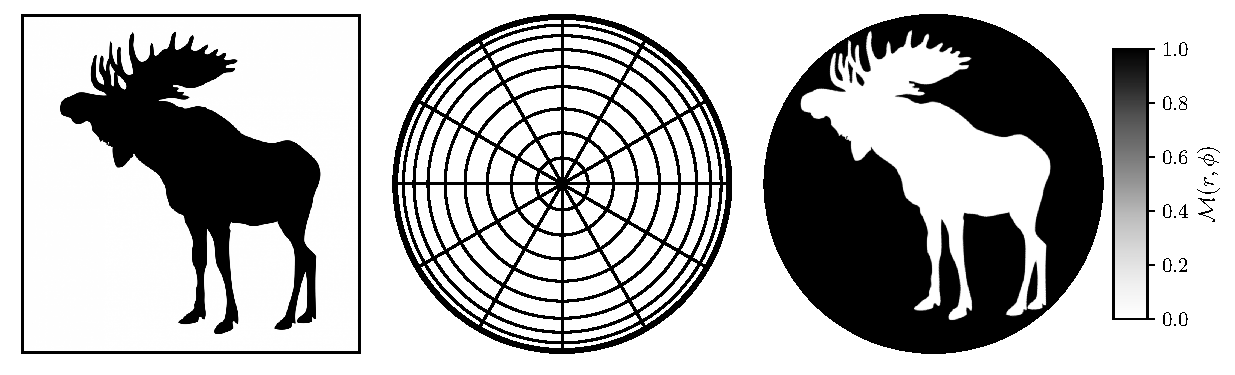
\includegraphics[width=\textwidth]{paper_figure01.pdf}
    \caption{ 
        (Left) A public-domain silhouette of a moose.
        (Middle) A sparse representation of the polar-coordinate grid on which we represent fields in our simulation.
        (Right) The Moosinesq mask $\mathcal{M}$ felt by our equations; fluid motions are damped where $\mathcal{M} > 0$.
        \label{fig:methods}
    }
\end{figure*}

We nondimensionalize Eqns.~\ref{eqn:incompressible}-\ref{eqn:temperature} and evolve them in time using the Dedalus\footnote{Ironically we did not the \texttt{MOOSE} simulation framework (\url{https://mooseframework.inl.gov/}). Sorry.} \citep{burns_etal_2020} pseudospectral solver.
Details of the nondimensionalization and simulation can be found in appendix~\ref{app:nondim_equations}.
The simulation presented in this work was run at a Rayleigh number of Ra = $10^{11}$ and a Prantler number of Pr = $1$.
The code used to the run simulations is available online in a github repository\footnote{\url{https://github.com/evanhanders/moosinesq_convection}}.
